\documentclass[titlepage]{article}


\usepackage{fancyhdr}
\usepackage{url}
\usepackage{tikz}
\usepackage{caption}

\pagestyle{fancy}

\fancyhead[L]{\thepage}



\title{Computer Workshop\\Assignment 2: Core Git}
\author{Dr. MalekiMajd}
\date{Due: 6 Azar, 1402}

\newcommand{\code}{\texttt}

\begin{document}
\maketitle

\section*{Assignment Notes:}
\begin{enumerate}
    \item Some questions may include material not yet covered in class. These questions are meant to help you develop your research skills.
    \item Cheating or copying homework is strictly forbidden. If caught, both students involved will receive a score of 0 on this assignment.
    \item If you have any questions, feel free to ask in the course's Telegram group to benefit your fellow classmates.
    \item It's recommended to visit Git's official documentation for additional information on its commands.
\end{enumerate}

\pagebreak

\section{More Git commands}
\subsection{Cloning}
In this section, you will be learning about a core feature in Git called \textit{cloning}. read about
cloning and answer the following questions:
\begin{enumerate}
    \item What does cloning a repository mean?
    \item What is the command for cloning a GitHub repository?
    \item Does cloning a repository retain its commit history?
\end{enumerate}

\subsection{Forking in Open-Source Projects and GitHub}

In this section, you will explore the concept of \textit{forking} in the context of open-source projects on GitHub. Read about forking and answer the following questions:

\begin{enumerate}
    \item What does it mean to fork a repository on GitHub?
    \item Describe the process of forking a repository.
    \item How does forking contribute to collaborative development in open-source projects?
    \item After forking a repository, how can you keep your fork up-to-date with the original repository's changes?
\end{enumerate}

\subsection{Git Resetting}

In this section, you will delve into the Git command \texttt{git reset}. Read about Git resetting and answer the following questions:

\begin{enumerate}
    \item What is the purpose of the \texttt{git reset} command in Git?
    \item Describe the difference between \texttt{git reset} and \texttt{git revert}.
    \item Explain the three primary modes of \texttt{git reset} (\texttt{--soft}, \texttt{--mixed}, and \texttt{--hard})
        and how they affect the staging area and working directory.
\end{enumerate}

\pagebreak

\section{Merging and Rebasing}
In this section, you will be given a GitHub URL that contains a repository that you need to fork and
make your own necessary changes on them and push them to your own GitHub repository.

Repository URL: \url{https://github.com/MiliAxe/cw1402_proj/tree/master}

Follow the necessary instructions on the projects given below.


\subsection{First project}
In this project, you are given a project that consists of three branches called master (main branch), feature-one and bug-fix. You have to first merge bug-fix into feature-one and after that, merge the branch feature-one into master.

Here is a demonstration of how this project looks like:

\begin{figure}[ht]
    \centering
    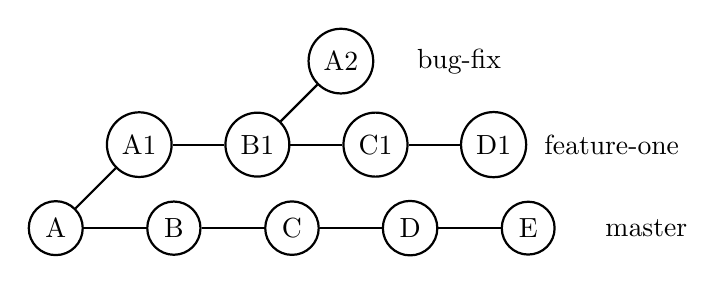
\begin{tikzpicture}[node distance={15mm}, thick, main/.style = {draw, circle}] 
        \node[main] (A) {A};
        \node[main] (B) [right of=A] {B};
        \node[main] (C) [right of=B] {C};
        \node[main] (D) [right of=C] {D};
        \node[main] (E) [right of=D] {E};
        \node[below left] (master) [right of=E] {master};
        
        \node[main] (A1) [above right of=A] {A1};
        \node[main] (B1) [right of=A1] {B1};
        \node[main] (C1) [right of=B1] {C1};
        \node[main] (D1) [right of=C1] {D1};
        \node[below left] (master) [right of=D1] {feature-one};
        
        \node[main] (A2) [above right of=B1] {A2};
        \node[below left] (master) [right of=A2] {bug-fix};
        
        \draw (A) -- (B);
        \draw (B) -- (C);
        \draw (C) -- (D);
        \draw (D) -- (E);
        
        \draw (A) -- (A1);
        \draw (A1) -- (B1);
        \draw (B1) -- (C1);
        \draw (C1) -- (D1);
        
        \draw (B1) -- (A2);
    \end{tikzpicture}
    \caption{Project 1}
    \label{fig:project1-before}
\end{figure}

After merging the branches, your project should look like this:
\begin{figure}[ht]
    \centering
    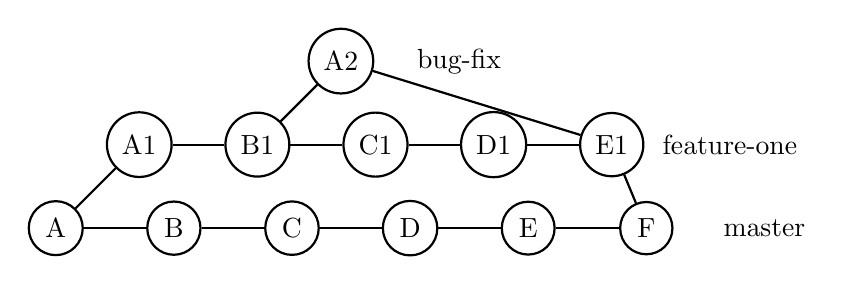
\begin{tikzpicture}[node distance={15mm}, thick, main/.style = {draw, circle}] 
        \node[main] (A) {A};
        \node[main] (B) [right of=A] {B};
        \node[main] (C) [right of=B] {C};
        \node[main] (D) [right of=C] {D};
        \node[main] (E) [right of=D] {E};
        \node[main] (F) [right of=E] {F};
        \node[below left] (master) [right of=F] {master};
        
        \node[main] (A1) [above right of=A] {A1};
        \node[main] (B1) [right of=A1] {B1};
        \node[main] (C1) [right of=B1] {C1};
        \node[main] (D1) [right of=C1] {D1};
        \node[main] (E1) [right of=D1] {E1};
        \node[below left] (master) [right of=E1] {feature-one};
        
        \node[main] (A2) [above right of=B1] {A2};
        \node[below left] (master) [right of=A2] {bug-fix};
        
        \draw (A) -- (B);
        \draw (B) -- (C);
        \draw (C) -- (D);
        \draw (D) -- (E);
        \draw (E) -- (F);
        
        \draw (A) -- (A1);
        \draw (A1) -- (B1);
        \draw (B1) -- (C1);
        \draw (C1) -- (D1);
        \draw (D1) -- (E1);
        \draw (E1) -- (F);
        
        \draw (B1) -- (A2);
        \draw (A2) -- (E1);
    \end{tikzpicture}
    \caption{Project 1 after merging}
    \label{fig:project1-after}
\end{figure}

\paragraph{NOTE:}
In case of any conflicts, keep the content of both of the branches.

\subsection{Second project}
In this project, you are given a project that consists of three branches called master (main branch), feature-one and bug-fix. You have to rebase bug-fix into feature-one and after that, rebase the branch feature-one into master.

Here is a demonstration of how this project looks like after and before rebasing:

\begin{figure}[ht]
    \centering
    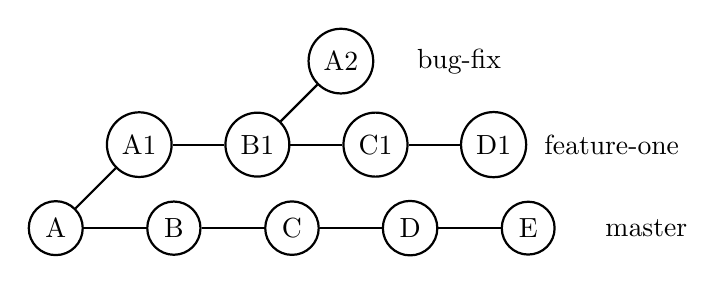
\begin{tikzpicture}[node distance={15mm}, thick, main/.style = {draw, circle}] 
        \node[main] (A) {A};
        \node[main] (B) [right of=A] {B};
        \node[main] (C) [right of=B] {C};
        \node[main] (D) [right of=C] {D};
        \node[main] (E) [right of=D] {E};
        \node[below left] (master) [right of=E] {master};
        
        \node[main] (A1) [above right of=A] {A1};
        \node[main] (B1) [right of=A1] {B1};
        \node[main] (C1) [right of=B1] {C1};
        \node[main] (D1) [right of=C1] {D1};
        \node[below left] (master) [right of=D1] {feature-one};
        
        \node[main] (A2) [above right of=B1] {A2};
        \node[below left] (master) [right of=A2] {bug-fix};
        
        \draw (A) -- (B);
        \draw (B) -- (C);
        \draw (C) -- (D);
        \draw (D) -- (E);
        
        \draw (A) -- (A1);
        \draw (A1) -- (B1);
        \draw (B1) -- (C1);
        \draw (C1) -- (D1);
        
        \draw (B1) -- (A2);
    \end{tikzpicture}
    \caption{Project 1}
    \label{fig:project2}
\end{figure}

\begin{figure}[ht]
    \centering
    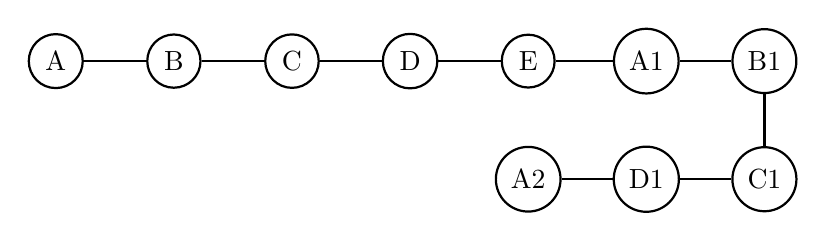
\begin{tikzpicture}[node distance={15mm}, thick, main/.style = {draw, circle}] 
        \node[main] (A) {A};
        \node[main] (B) [right of=A] {B};
        \node[main] (C) [right of=B] {C};
        \node[main] (D) [right of=C] {D};
        \node[main] (E) [right of=D] {E};
        % \node[below left] (master) [above of=E] {master};
        
        \node[main] (A1) [right of=E] {A1};
        \node[main] (B1) [right of=A1] {B1};
        \node[main] (C1) [below of=B1] {C1};
        \node[main] (D1) [left of=C1] {D1};
        % \node[below left] (master) [below of=D1] {feature-one};
        
        \node[main] (A2) [left of=D1] {A2};
        % \node[below left] (master) [left of=A2] {bug-fix};
        
        \draw (A) -- (B);
        \draw (B) -- (C);
        \draw (C) -- (D);
        \draw (D) -- (E);
        
        \draw (E) -- (A1);
        \draw (A1) -- (B1);
        \draw (B1) -- (C1);
        \draw (C1) -- (D1);
        
        \draw (D1) -- (A2);
    \end{tikzpicture}
    \caption{Project 2 after rebasing}
    \label{fig:project2-after}
\end{figure}

\paragraph{NOTE:}
In case of any conflicts, keep the content of both of the branches.

\subsection{Instructions}
For better understanding of what should be done in this section, here are some instructions:
\begin{enumerate}
    \item Head to the GitHub URL provided
    \item Fork the repository provided and rename the repository to the format \texttt{HW\_STUDENTNO}
    \item Apply the necessary changes stated in the sections.
    \item Push the changes to your forked repository
    \item Provide the URL to your GitHub repository in your assignment's PDF as well as the commands you
        applied on the repository.
\end{enumerate}

\end{document}

